% LaTeX Template for Project Report, Version 2.0
% (Abstracted from a Major Project Report at CSED, NIT Calicut but can be
% modified easily to use for other reports also.)
%
% Released under Creative Commons Attribution license (CC-BY)
% Info: http://creativecommons.org/licenses/by/3.0/
%
% Created by: Kartik Singhal
% BTech CSE Batch of 2009-13
% NIT Calicut
% Contact Info: kartiksinghal@gmail.com
%
% It is advisable to learn the basics of LaTeX before using this template.
% A good resource to start with is http://en.wikibooks.org/wiki/LaTeX/
%
% All template fields are marked with a pair of angular brackets e.g. <title here>
% except for the ones defining citation names in ref.tex.
%
% Empty space after chapter/section/subsection titles can be used to insert text.
%
% Just compile this file using pdflatex after making all required changes.

\documentclass[12pt,a4paper]{report}
\usepackage[pdftex]{graphicx} %for embedding images
\usepackage{url} %for proper url entries
\usepackage[bookmarks, colorlinks=false, pdfborder={0 0 0}, pdftitle={A Visual Programming Environment for Novices}, pdfauthor={Mark Provan}, pdfsubject={<subject here>}, pdfkeywords={<keywords here>}]{hyperref} %for creating links in the pdf version and other additional pdf attributes, no effect on the printed document
%\usepackage[final]{pdfpages} %for embedding another pdf, remove if not required

\begin{document}
\renewcommand\bibname{References} %Renames "Bibliography" to "References" on ref page

%include other pages
\begin{titlepage}

\begin{center}

\textup{\small {\bf CS4099 Project} \\ Report}\\[0.2in]

% Title
\Large \textbf {A Visual Programming Environment for Novices}\\[0.5in]

% Submitted by
\normalsize Submitted by Mark Provan

\vspace{.1in}
Under the guidance of\\
{\textbf{Edwin Brady}}\\[0.2in]

\vfill

% Bottom of the page

\includegraphics[width=0.18\textwidth]{sta-logo}\\[0.1in]
\Large{School of Computer Science}\\
\normalsize
\textsc{University of St Andrews}\\
St Andrews, Fife, Scotland \\
\vspace{0.2cm}
Candlemas Semester 2017

\end{center}

\end{titlepage}

\vspace{2in}
\begin{abstract}



\end{abstract} 

\newpage
\thispagestyle{empty}

\begin{center}

\huge{School of Computer Science}\\[0.5cm]
\normalsize
\textsc{University of St Andrews}\\[2.0cm]

\emph{\LARGE Declaration}\\[2.5cm]
\end{center}
\normalsize I declare that the material submitted for assessment is my own work except where credit is explicitly given to others by citation or acknowledgement. This work was performed during the current academic year except where otherwise stated. The main text of this project report is 18,199 words long, including project specification and plan. In submitting this project report to the University of St Andrews, I give permission for it to be made available for use in accordance with the regulations of the University Library. I also give permission for the report to be made available on the Web, for this work to be used in research within the University of St Andrews, and for any software to be released on an open source basis. I retain the copyright in this work, and ownership of any resulting intellectual property.\\[1.0cm]

\vfill

\pagenumbering{roman} %numbering before main content starts
\tableofcontents
\listoffigures

\newpage
\pagenumbering{arabic} %reset numbering to normal for the main content

\chapter{Introduction}

\section{Overview}

\section{Aims and Objectives}
\subsection{Primary}

some text\cite{citation-1-name-here}, some more text
\subsection{Secondary}

even more text\footnote{<footnote here>}, and even more.
\subsection{Tertiary}

\section{Key aspects} %literature survey included in this
\chapter{Context Survey}

\section{Programming Education}

\section{Visual Programming for Novices}

\section{Comparable projects and inspiration}

\subsection{Scratch}

\subsection{Lamdu}

\subsection{Learnable Programming by Brett Victor}
 %objective changed to problem definition
\chapter{Ethics}

No user studies have been performed so there are no ethical concerns with this project. However, in the initial planning of this project there was the possibility that such studies could have been undertaken, so ethical approval was sought and granted.
\chapter{Design}

\section{Program visualisation}

\subsection{Traditional programming model}

\paragraph{Lexing}

\paragraph{Parsing}

\subsection{Abstract Syntax Tree visualisation}

\subsection{AST editing}

\paragraph{Insertion of new elements}

\section{Program change tracking}

\section{Program execution}

\subsection{Interpreter option}

\subsection{Trans-compilation option}

\subsection{Virtual machine option}

\subsubsection{Concept}

\subsubsection{Implementation}

\subsection{Virtual machine formal specification}

\subsubsection{Machine}

\subsubsection{Instruction set}

\subsection{Code generation, labelling and AST-instruction mapping}

\subsection{Method call interface}

\section{Program input and output}

\section{Language specification}

\section{Platform independence}


\chapter{Implementation}

\section{Web application}

The programming environment is implemented as a web application capable of running within any modern or future web browser. The application is entirely self-contained and has no dependency upon an internet connection or access to servers. However, unlike traditional web development the initial source code is not the final executed product. Instead a series of modern tools, frameworks and technologies are used to transform TypeScript and React framework source code into standards-compliant JavaScript and HTML.

While the final application will be able to run in any backwards-compliant web environment it is possible that the tools and frameworks needed to modify and build it may become obsolete. The rapid pace of web development technology in recent years has seen entire tools developed, used and then replaced by newer and better versions. Rejecting the use of these tools due to their possible future obsolescence would be inappropriate. So far, all technology frameworks used to create programming language education and visualisation tools have ever been deprecated or become less significant with time, even in the case of Java and its 'write-once, run-anywhere' philosophy. While some web tools have become obsolete, they are all open-source technology and so are not dependent upon the good grace of a commercial enterprise to be maintained and kept available. A development tool that targets the universal web platform has a better chance of being kept usable in future than a tool which targets a closed and/or decaying platform. In addition, these tools are all themselves implemented using web technologies of some variety. All of the tools used to create the final compiled application run within the Node.js platform, which is a non-browser implementation of a JavaScript programming environment. Any development effort into the web as a platform also applies to Node.js and vice-versa.

JavaScript is the standard scripting language for use in the web platform. Developed by Brendan Eich in only ten days\cite{6155645}, the language was never designed for the vast range and scale of applications that now run in modern web browsers. With the web having exploded in popularity it has been impossible to replace it in the browser with something inherently more suited for modern web applications. The language is extremely flexible in allowing a wide range of programming styles, from standard sequential programming to object-oriented and functional uses. The standard has developed over time to include more features but without breaking backwards-compatibility. These new features have often consisted of syntactic sugar over complicated existing implementations, such as the new class definition syntax which allows object-oriented code to be written in a style similar to that in Java or other OOP languages. With the underlying compatibility between the new features and existing JavaScript implementations, it has been possible for tools to take in a modern version of JavaScript and then output some older version which will run on a much wider range of current and old browser versions with no change of functionality.

While these new features have assisted programmers in creating large applications, the language remains untyped. Without types, it is hard to statically reason about the correctness of a program such that bugs are found without extremely exhaustive (i.e. expensive) testing, or worse by end-users. TypeScript is a new language developed as open-source by Microsoft to solve this problem. As with the JavaScript version converters, all TypeScript code is translated into standards-compliant JavaScript that may run in any existing implementation. TypeScript is a pure superset of the most modern JavaScript standard with the enhancement that the programmer has the choice to specify types. It is therefore perfectly suited for the role of large-scale web application development, and so I chose to use it for this project.

\section{User interface}

\subsection{React framework}

The user interface for this tool requires dynamic creation of visual elements which possess common visual and behavioural elements. The web platform fundamentally works through the Document Object Model, where elements on a web page are structured in a tree. All elements may define attributes such as their text content or any functions that should be called upon certain events occurring to them. HTML is an efficient method to define these DOM nodes in a static manner, but it cannot generate nodes dynamically based upon programmed behaviour. JavaScript code in the browser may interact with the DOM to insert, delete and modify elements as required by any other parts of the code. Modifications to the DOM may be interspersed at arbitrary locations in the JavaScript code of a web page. Styles can be applied to the DOM nodes using either a static CSS file or dynamically through JavaScript; the browser renders the nodes according to these rules without the underlying representation of the DOM being changed.

The traditional HTML, JavaScript and CSS model is sufficient for basic web pages and applications, but does not scale with increasing application size. Adding additional composable parts of the application requires increasing effort. As with all programming, the more code that needs written, the more chance of things going wrong. To avoid the need to spend significant amounts of time debugging basic rendering code, I decided to use a modern web application framework for the user interface of this application. There are a number of such frameworks available for use, all free and open source for anyone to make use of in their own time despite being largely written by and for the largest of web application companies such as Facebook and Google.

After writing the initial prototypes using raw DOM manipulation, I chose the React framework. While some frameworks such as Angular aim to simplify the creation of the entire application with features such as application routing (where the browser URL updates as the web application is navigated despite no new pages being requested from the web server), React is designed to implement only the visual presentation layer. It implements the view side of the Model-View-Controller concept and is designed around a functional approach to rendering DOM components based upon a given application state\cite{Gackenheimer2015}. Every time the application state is changed, the entire application is re-rendered functionally. However, this rendering is done in a Shadow DOM and only once complete the difference between the old and new forms is calculated and the most minimal changes applied to the real browser DOM to bring it up to date.

The user interface is defined as a series of React components. React components define a \verb+render+ method which return a React-specific representation of the component DOM structure. This representation can either be created using pure JavaScript (or TypeScript)\footnote{The basic functionality of React is the same in both JavaScript and TypeScript. React is aware of TypeScript and provides types for its type checking systems, but otherwise does not provide any extra functionality. I therefore describe React in how it works with JavaScript, despite using it with TypeScript in this project.} using React library methods or in JSX (TSX), which is an extension of the JavaScript language to include XML-style blocks. The JSX representation is simply syntactic sugar for the library function call method and an early step in the compilation process converts JSX code to this form. The JSX form allows for component structures to be defined in a form very similar to HTML, making it ideal for use in the toy language specification as a language designer will not need significant training to produce the visual representation of their language. React rendering of components is done by recursive descent; components may include other full components within them alongside standard DOM nodes and text content.

\subsection{App}
Implementing the Model-View-Controller framework correctly requires that changes to the model are done through one single mechanism - the controller. The entire state of the program is represented through an App instance, which includes controller methods to change the state in a controlled manner. These changes include:
\begin{itemize}
\item Editor undo/redo
\item Execute forward/backward one step
\item Replace AST node element
\item Delete/insert/replace AST node element from/into/in parent node array
\end{itemize}

Upon one of these changes being requested, the App instance will perform that change and then cause the entire user interface to be re-rendered within the React framework.

\subsection{AST and editor}

In the toy language specification, each AST node type must defined its own \verb+render+ method which returns the React component for that node type. This node type extends from a common base React component, which implements language and structure-agnostic functionality. This includes selecting nodes by clicking (which causes a visual effect and causes the instructions generated from that node to be highlighted) and the visual expansion and display of the node type name that occurs when the user mouses over it.

The concrete implementation of the node component includes the \verb+getInnerElement+ method to generate the node-specific contents of that component. This content can be in any arbitrary design or structure to allow simple visual representation of the AST node. However, keywords and syntax elements (such as brackets and symbols) are displayed using common component types. These components are:
\begin{itemize}
\item \textit{ButtonComponent}
\item \textit{KeywordComponent}
\item \textit{SyntaxComponent}
\item \textit{VerticalListComponent}
\item \textit{HorizontalListComponent}
\end{itemize}
These common components allow each language to be displayed and interacted with in a standardised way. Each node type defines how it should be displayed in the UI, using a combination of the generic components. A key visual differentiator between different node types is the use of block colour, and the language specification includes a stylesheet which can apply any arbitrary web styling to the node representation. So far this has only been used for colours but it would be trivial to specify a different border or shape as well.

\paragraph{Child AST node components}
The child node components are not added directly but instead through a wrapper component type, which is passed the reference to the child node as well as the methods required to modify it. A wrapper exists for each of the basic language types (such as expression and statement in the \textit{lang} toy language). This is necessary for there to be common handling of inserting, deleting and editing child nodes across all instances of that type. If the child AST node does not exist, the wrapper component provides the means to add a valid node of that type such as the keyboard entry and selection menu.

When the user makes a change using this wrapper component, the callback provided in the parent component is used to effect that change. For example, the parent component may generate a JavaScript closure function to include the index of the array in which the element is located for the array editing calls provided by \textit{App}. This flexibility allows for wrapper components to be used regardless of the structure of the parent node. There can arbitrary numbers of same element types within a node, so long as they have some unique reference by name or array name and index.

The program editor itself is a simple wrapper component around the entire AST. With a significant proportion of the editing systems implemented through common components within the AST rendering, this component is itself only responsible for the undo and redo buttons. These buttons call through to equivalent operations on the \textit{App} object as a whole.

\subsection{Instructions and machine state}

The remainder of the user interface is dedicated to represent the state of the virtual machine. Each separable part of the machine state has its own component. User interaction is limited primarily to the Backward and Forward buttons which cause the machine to run one step in that direction. 

\subsubsection{Instructions}

The Instructions component displays a list of all of the instructions loaded into the virtual machine. Each instruction is displayed with its own component, which displays the relevant information for each instruction type as appropriate. The component of the instruction currently being executed is highlighted in the same colour as the corresponding AST node to provide the visual link between the program code and the generated instructions. Each instruction displays a small list of the AST nodes which led to its generation, and these small node reference components can be clicked to highlight that node and its instructions. This small component is also used in the display of local labels on the left hand side of the instruction listing. The global labels of the machine are used as visual dividers between different instruction ranges, while otherwise their appearance remains the same and the numbering remains consistent.

\subsubsection{Stack Frames and Global Environment}

The stack component simply presents a visual metaphor for the state of the stack. Each stack frame is presented in order as its own component, each of which shows its stack elements in order as individual blocks. The return address in that stack frame is shown, if available, and the contents of the key-value \textit{Environment} are displayed visually.

The global environment is shown in a similar manner to the stack frame environment, albeit in a separate component and without being contained within a stack frame.

\subsubsection{Console}

The console component is relatively simply, in that it only needs to display the text content included in the Console machine part. While output works as normal, input is made difficult by the non-blocking nature of JavaScript. The \textit{ConsoleIn} instruction semantics are blocking but there is no simple way to pause program execution while waiting for the user to enter an input into a complex, JavaScript-implemented text console. As a result, the standard JavaScript \verb+prompt+ method is used to open a browser dialog box. This is blocking and so a result can be obtained without changes to the rest of the programming environment architecture.

\section{Program components}

\subsection{Machine}

The virtual machine is implemented as a TypeScript class. An instance of the VM includes:
\begin{itemize}

\item an array of Instruction objects
\item Representations of the stack, global environment and text console
\item standard key-value mapping objects in both directions between instruction labels and array indices
\item an array of all previous \textit{MachineChange} objects
\item a \textit{Map} between AST node instances and their instruction range
\item an array of currently active AST nodes at each instruction index.
\end{itemize}
The Machine class provides a number of different methods which are used within the AST code generation process to add an instruction or label, or to begin and end AST instruction ranges. When called, these methods add the necessary information to the records of instruction range and label mappings as appropriate in a single pass. Other methods are provided for the execution stage:

\begin{itemize}
\item \verb+applyMachineChange+ applies a given \textit{MachineChange} instance to the current object; it is the only mutative step in the entire execution process.
\item \verb+oneStepExecute+ and \verb+oneStepBackward+ perform a single round of instruction fetch (from the instruction pointer or from the reversed last performed operation) and execute.
\item \verb+getExecutingASTNode+ is used by the UI to highlight the current AST node.
\item \verb+canContinue+ and \verb+canReverse+ are used to enable and disable the Forward and Backward execute buttons.
\end{itemize}

\paragraph{Stack and StackFrame}

The stack object includes an array of StackFrame objects. Push, pop and get methods are provided for stack frames as well as push, pop and peek methods that act upon the topmost stack frame. In addition to the array of stack elements, a StackFrame also includes
\begin{itemize}
\item An Environment key-value mapping which is used to store named variables
\item A return address instruction pointer number
\item An array of arguments, used in the method call interface
\end{itemize}

\paragraph{Global Environment}

The global environment is a single \textit{Environment} instance which is used to store named variables which are shared between all parts of the program.

\paragraph{Console}

The console object is used to store and modify the current textual state of the machine console. This implements operations to add a set of characters to the end of the console text and to delete a set number of characters from the end of this text.

\subsection{MachineChange}

Changes to the machine state are represented as instances of the \textit{MachineChange} class. This class wraps a list of individual \textit{MachineComponentChange} instances alongside the change to the machine instruction pointer. Each type of individual change is represented as a subclass of \textit{MachineComponentChange}, which sets the specification of having an apply method which takes a given machine instance and then causes that change to be applied to it, and a reverse method which will return the inverted form of that change. The different possible changes are:

\begin{itemize}
\item \textit{StackPushChange}
\item \textit{StackPopChange}
\item \textit{StackFramePushChange}
\item \textit{StackFramePopChange}
\item \textit{GlobalEnvChange}
\item \textit{StackFrameEnvChange}
\item \textit{StackFrameChange}
\item \textit{ConsoleChange}
\end{itemize}

Each of these types encapsulates the necessary information for that change to be made and also to be reversed. The 'pop' changes, for example, will record those things that were popped from the stack, while the other changes will record the previous value of any deleted or modified attribute. The reversal methods create a new change object of the correct type with the before-after values swapped so that they may be applied directly to reverse the change. The entire \textit{MachineChange} has a \verb+reverse+ method which also creates a new \textit{MachineChange} object, with a reversed list of each reversed \textit{MachineComponentChange} plus the negation of the instruction pointer change.

\subsection{Instruction}

Each virtual machine instruction is represented as a subclass of the abstract Instruction class, implementing the abstract \verb+machineChange+ method which takes in a while Machine instance and produces a single \textit{MachineChange} object. Each instruction type class includes the operands of that instruction, which are then used during in the \verb+machineChange+ method implementation to calculate the real change to the machine. A \textit{CallFunction} instruction contains a \textit{MachineFunction} instance, which wraps a standard JavaScript function with its name and arity\footnote{The arity of a function is the number of arguments that it takes}. The \verb+machineChange+ method pops the arity number of values off the stack into an array, which is then passed as a set of arguments to the wrapped function using the JavaScript function \verb+apply+ method. The actual computed return value is captured in a singleton array, which then forms the array of elements pushed on the stack in the \textit{MachineChange}.

\section{Parsing}

The \textit{PEG.js} library provides for parsing of textual program representations. This parsing is done on the example code that is loaded along with a language definition, and in the textual new node input system. This library uses its own version of a grammar definition \cite{pegjs}, which is used with a parser generator to create an optimised parser object for that exact grammar. This grammar definition can include JavaScript code to be evaluated and returned upon the match of a grammar type; this is used to create instances of each of the toy language node types. Using a library for this allowed for work to be concentrated on the novel aspects of the project, but came at the cost of it being less than well optimised for this exact use case.

As an example, it is necessary to attach the language definition file to the global \verb+window+ scope so that the grammar JavaScript code can use it. In early development versions of this practical, the language definition code was transformed from TypeScript into JavaScript separately and then inserted into the grammar files before being used. This meant that the browser did not consider grammar-created objects to be of the same class as those created elsewhere.

At this point in time, the parser is not able to perform auto-correct, and can only return an element if the entire input is complete and valid.
\chapter{Evaluation and Critical Appraisal}

Programming education is clearly a very hard subject area, combining the general complexity of education itself with the need to explain and teach the workings of a thinking ‘mind’ that has been only a recent addition to human civilisation. Programming education is a research field in itself, and so it is unlikely that this one tool will be some holy grail which will solve all problems. However, in terms of the original goals of combining visualisation, enforced program correctness and being able to act as a platform for different programming styles I believe this project has been a success.

In my opinion, a key part of that success is due to the focus on representing only the most basic aspects of programming, those which give the novice learner enough understand to then go on and tackle the more complicated topics. While I have described the problems with a text-based model of programming for some users, I do not believe that it is at all an inappropriate model to use for skilled programmers. As such, there is no requirement to implement all of the features that a real-world programming environment would require. Limiting the scope of the system in this manner means that I have been able to concentrate on the novel aspects that will actually help novices.

Despite the focus on novices, what I have found very interesting in the course of this project is how the systems that I implemented to help novices could in fact be used as well to aid more experienced programmers as they learn the art of computer science. In particular, the visualisation of how any arbitrarily complex program is transformed into a linear series of instructions would demonstrate the nature of compilers. The instruction list was not included in my original plans for this project, as I believed initially that the program code would be evaluated and not run on a virtual machine. However, with the instructions being displayed during development it became clear that they should form a vital part of the user interface.

\section{Toy languages implemented}

\subsection{lang}

This language is a simple procedural language with a limited number of constructs. It was the initial single embedded toy language used to test and create the environment. It supports basic variable assignment and retrieval from a local stack frame, loops in the while statement, using method calls as an expression and returning values from a method.

\begin{figure}[htb]
\centering
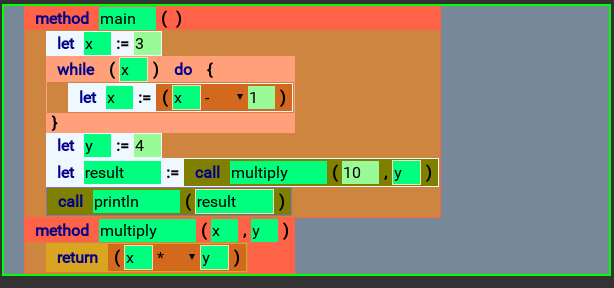
\includegraphics[scale=0.5]{graphics/langprog} % e.g. insert ./image for image.png in the working directory, adjust scale as necessary
\caption{Example of a \textit{lang} program}
\label{fig:langprog} % insert suitable label, this is used to refer to a fig from within the text as shown above
\end{figure}

\begin{figure}[H]
\centering
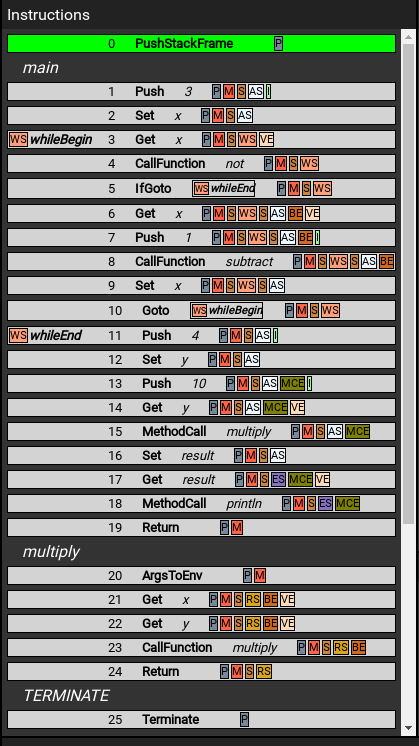
\includegraphics[scale=0.5]{graphics/langcode} % e.g. insert ./image for image.png in the working directory, adjust scale as necessary
\caption{Sample of code generated from the \textit{lang} program in Figure \ref{fig:langprog}}
\label{fig:langcode} % insert suitable label, this is used to refer to a fig from within the text as shown above
\end{figure}

\begin{figure}[H]
\centering
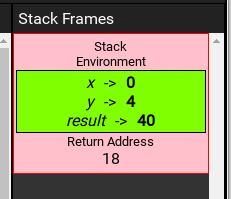
\includegraphics[scale=0.5]{graphics/langstack} % e.g. insert ./image for image.png in the working directory, adjust scale as necessary
\caption{Machine stack after executing the \textit{lang} program in Figure \ref{fig:langprog}}
\label{fig:langstack} % insert suitable label, this is used to refer to a fig from within the text as shown above
\end{figure}

\begin{figure}[H]
\centering

\includegraphics[scale=0.5]{graphics/langconsole} % e.g. insert ./image for image.png in the working directory, adjust scale as necessary
\caption{Console text after executing the \textit{lang} program in Figure \ref{fig:langprog}}
\label{fig:langconsole} % insert suitable label, this is used to refer to a fig from within the text as shown above
\end{figure}

\subsection{fun}

This language is a rudimentary purely functional language where all execution consists of evaluation. It does not support higher-order functions but it serves a purpose of contrasting the pure evaluation approach against the statefulness of a procedural language. It also demonstrates the concept of recursion, as is used in the example program to calculate a Fibonacci and a factorial number using the basic recursive definitions of both algorithms. Its functional nature extends to the trace standard library method, which behaviours similarly to the same-named function in Haskell's debugging libraries in that it is given an extra argument that it will evaluate to as well as having the side-effect of writing text output.

\paragraph{Errata} the language grammar does not support anything other than addition, multiplication, division and subtraction for binary expressions. However, the language definition in code allows for numerical comparison and the AND and OR binary operators. These may be selected using the user interface but cannot be included in the textual form of a program. As these are required for the Fibonacci and factorial algorithms, while the pre-loaded test programs have to be parsed from their text form, it is currently necessary for the user to manually change the binary operator to \verb+<=+ from \verb+\++ after loading the test program.

\begin{figure}[H]
\centering
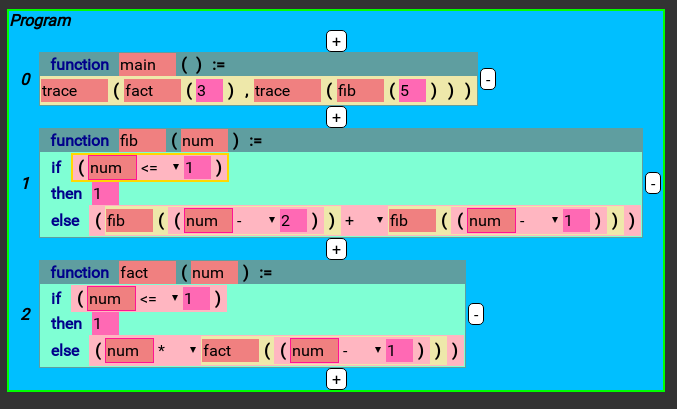
\includegraphics[scale=0.5]{graphics/funprog} % e.g. insert ./image for image.png in the working directory, adjust scale as necessary
\caption{Example of a \textit{fun} program}
\label{fig:funprog} % insert suitable label, this is used to refer to a fig from within the text as shown above
\end{figure}

\begin{figure}[H]
\centering
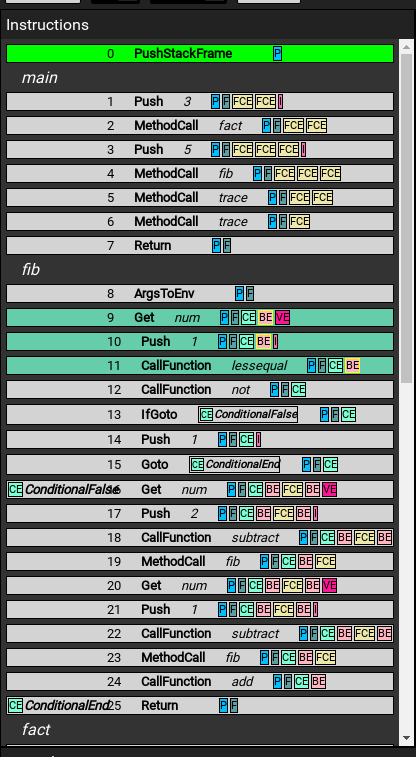
\includegraphics[scale=0.5]{graphics/funcode} % e.g. insert ./image for image.png in the working directory, adjust scale as necessary
\caption{Sample of code generated from the \textit{fun} program in Figure \ref{fig:funprog}}
\label{fig:funcode} % insert suitable label, this is used to refer to a fig from within the text as shown above
\end{figure}

\begin{figure}[H]
\centering

\includegraphics[scale=0.5]{graphics/funconsole} % e.g. insert ./image for image.png in the working directory, adjust scale as necessary
\caption{Console text after executing the \textit{fun} program in Figure \ref{fig:funprog}}
\label{fig:funconsole} % insert suitable label, this is used to refer to a fig from within the text as shown above
\end{figure}

\section{Comparison against original objectives}

\subsection{Primary}

\begin{itemize}
\item Create a web application - \textbf{Done}
\item The application must allow the user to write programs - \textbf{Done}
\item The writing of these programs will be done straight into a visual representation of the language's abstract syntax tree - \textbf{Done}
\item The programs must be able to be run within the application - \textbf{Done}
\end{itemize}

All four primary objectives have been completed. I believe that their design and implementation is solid, and provide a good platform for future work.

\subsection{Secondary}

\begin{itemize}
\item The execution of these programs must be shown visually with relevant feedback - \textbf{Done}
\subitem e.g. showing the steps of evaluating an expression
\item The execution must be able to be paused and rewound at any time - \textbf{Done}
\item Code changes must be able to be done at any time - Mostly done
\item There will be some way for the programs to have input and output - \textbf{Done}
\item There will be multiple types of possible program input and output - \textbf{Not done}
\subitem e.g. drawing on a canvas, inputting/outputting tabular data
\item There will be several different programming concepts/styles supported - \textbf{Done}
\subitem e.g. functional, scripting, object-oriented, bare-metal
\item Multiple tweaked versions of the program will be able to run in parallel to visually demonstrate algorithmic differences between them - \textbf{Not done}
\end{itemize}

A number of the secondary objectives have been completed in full. Again, I believe that my design and implementation of these is solid. Of the tasks not completed fully, many are well within reach with only minimal extra work due to the strong foundation of the rest of the application.

For example, being able to perform code changes at any time is mostly done, as AST changes can be performed at any time and they will have an immediate effect upon the generated instructions. However, it is not possible for changes to happen before the current node, as the instruction pointer is not re-calculated. If the number of instructions changes, the current instruction may change inadvertently and so the behaviour of the program affected. However, this should be an easy fix as a two-way mapping between AST nodes and their instruction ranges is already available. Supporting this feature would simply require finding the new instruction address of the current AST node.

Having multiple types of input and output was a significant goal of mine in my original plans for this project, as I drew heavily upon Brett Victor's \textit{Learnable Programming} ideas. I believed that it would be a good idea to implement his concept of a drawable canvas which supported the full reversibility and live code change features. This feature would be useful for novices learning for their own pleasure, as a great deal of satisfaction can be gained from creating a visual product. Tabular data would be more useful for novices who are working within the realms of the numerate sciences, as they may wish to learn how to program in order to process their own experimental or other data. Implementing these two systems would some work but it could build upon the existent console text input/output system. One possibility could be to implement input and output in a modular fashion so that advanced users or educators could implement arbitrary IO to suit their own needs. This may be particularly useful for the sciences where an IO module could be written to support a specific file type better than an entirely generic file reading one could.

Allowing multiple tweaked versions of the code to exist in parallel should be relatively straightforward given the strongly object-oriented and encapsulated implementation of the environment. An entire machine instance could be copied and so run in parallel without affecting the original. Including all of the information on screen at once may prove to be more of a challenge, as the full effect of a change may only be properly seen by showing all of the machine state of both programs as they execute.

\subsection{Tertiary}

\begin{itemize}
\item Multiple users will be able to work collaboratively on programs - \textbf{Not done}
\item It will be possible to export the program to a professional and compatible programming tool - \textbf{Not done}
\subitem - e.g. export to Python for scripted, Java for object-oriented, Haskell for functional
\item The visual representation of the code can be changed to represent higher-level concepts - \textbf{Not done}
\subitem e.g. object-oriented to UML
\end{itemize}

Unfortunately none of these three tertiary objectives has been implemented. However, a clear path to implementation is available for collaborative working due to the use of AST change diffs. The WebSocket API provides modern web browsers with real-time two-way message channel system that could be used to send and receive these change diffs from a centralised collaboration server.

The specification for toy languages could be extended to include export steps for suitable real programming languages. This code generation could be done in a similar recursive descent fashion to the virtual machine instruction generation, with generation methods defined for each AST node type for each different target language. The intention of this language export feature would be to preserve the structure and behaviour of the original problem, so it must be supported at a language level rather than being common to all languages. The reason for export would be to allow novices to continue working on any programs that they might write once they have reached a reasonable level of competency. Exporting a sequential toy language to a valid Haskell program with the same behaviour would be possible, but the produced code would be effectively unrecognisable.

The third tertiary requirement would be more challenging to implement. Again, these visual translations would need to be implemented at the language specification level as they would not be generic. The most likely course of action would be to implement a rendering API where the entire machine state would be provided and the language specification allowed to produce any visual elements that it requires.

\section{Critical appraisal}

\subsection{Achievements}

Overall, I am very pleased about the features that have been implemented. While many of the secondary and tertiary objectives have not been completed, it is clear that most of them are well within reach given extra time.

In particular, I think that my project has proved that the area of visual-textual programming languages is worth exploring further. With Lamdu being the closest equivalent but hamstrung by its limited portability and tight binding to a single programming language, I think that this project has created something truly novel. Creating a totally new experience for something so fundamental for programming, and thus for almost every area of society, is an achievement in itself. This creation will be immediately accessible to the billions of people across the world with any form of internet access without being any more limited in what it can do versus a traditional native application. 

It is also an achievement that the process of implementing it has further opened my eyes to the possibilities of the tool and technologies. Some projects may sound promising in concept but as work goes into them, it is found that they will not be able to fulfil those goals. Instead of doors being opened, they can be slammed shut as things are found to be too hard, impossible or not worthwhile. Using this project as a starting block I feel that there is much still to be explored.

\subsection{Drawbacks and problems}

While the project as a whole has been a success, there are elements which I know to be less than complete and that have a significant impact upon the immediately usability of the tool.

\paragraph{Usability}

Most importantly, I know that there is a lot of work to be done in fine-tuning the behaviour of the editor so that it acts entirely naturally. At the moment, the way that AST nodes change size and appearance upon being moused over is animated and smooth but in a very simplistic, proof-of-concept way. I myself have had problems interacting efficiently with the tool, with buttons moving away from the cursor faster than I can click on them. Fixing this would require extensive studies into human-computer interaction as the AST user interface is somewhat novel and incomparable to existing code editors and applications. Making the UI act simply effortlessly will almost certainly require considerable complexity under the surface. It may even be worth considering the use of novel input techniques such as eye tracking so that the computer better understands what the user is interested in exploring visually. At one point during development I considered that a three-dimensional cursor might be required, as the visual nesting of blocks creates an effective third dimension and users would expect to be able to use directional commands to navigate their code. Implementing such a cursor would be an HCI challenge of its own. However, as with other future ideas for improvement, the solid implementation of this project should allow these user interface concerns to be handled entirely separately from the rest of the code. Implementing a new input mechanism would only require changes to the visualisation and user input handling, which are encapsulated completely within the rendering code.

\paragraph{Parsing}

The other key drawback is parsing. As explained in the Implementation section, an off-the-shelf parsing library is used to parse program text. This library is not set up to auto-complete code suggestions, and so inserting program elements with text does not fulfil the initial design vision. Supporting auto-completion properly is very important for the usability of this tool, especially as the user becomes more confident and uses more keyboard input than cursor selections.

\section{Future directions}

\subsection{User studies}

While this tool fulfills many of the original objectives, its actual use for its initially-conceived purpose of programming education can only be determined by testing it out upon novice programmers. A normal application or tool may have its effectiveness examined by discovering how users interact with it in individual settings, as it does not require any long-term effort on the part of the test taker. In the initial planning stages of this project I expected to perform basic user studies in order to gain some feedback on how well the tool performed. However, as the project progressed it became clear that testing a tool of this nature would be a project unto itself given its educational basis. 

\paragraph{Evaluation by educators}
Determining whether or not it is useful for its target audience of novices would require tracking the progress of novice programmers as they learn using it as compared to a traditional programming education course. That many of the existing visualisation tools have been created by CS1 lecturers for use in their own classes is telling, as they are some of the few researchers in a position to track the progress of learners through their academic results and drop-out rates. If successive CS1 classes have proved to have a similar intake, experiences and then final results, then the effect of an educational tool can be determined by comparing the class-wide statistics against previous years. The testing of the tool can be done as part of the teaching of the CS1 course rather than in isolation as in a traditional user study. The effect of the tool may also be apparent in non-assessed coursework and lab time, as the sorts of questions and assistance that learners would ask about and request may change. A study on the effectiveness of the tool may therefore need to include notes and statistics on every teaching session. With the size of university CS1 classes growing and growing\cite{nager2016case}, performing such a comprehensive study would be a resource-intensive task. The full range of records would need to be kept when teaching using both the traditional methods and this new tool, further adding to the cost and complexity of a study.

\paragraph{Evaluation through massive open online courses}
A relatively low-resource possibility for a study would be to utilise the massive open online course (MOOC) concept, as the baseline teaching level is low and there is the possibility of recording usage analytics. Online coding platforms can easily record the time taken for a user to complete a task, the number of failed attempts and the rate at which a user progresses through different challenges. The location of the user's cursor and the rate at which they move it around could be treated as their focus location - a cursor left in a specific part of the code which is detected as incorrect would suggest that the user does not understand this part of their program. A more accurate, albeit more controversial, way to perform this user engagement tracking would be to make use of the webcam access APIs now available in modern browsers to perform focus tracking, to identify where the user is actually looking on the screen, as well as to analyse facial expressions for signs of engagement or disengagement.

These analyses could be applied to courses using both the traditional textual programming approach and to courses using this project's programming environment. Using the scale made possible by the MOOC concept, it should be possible to compare results for many hundreds or thousands of users. Long term tracking of performance would not be as straightforward as in a rigid academic setting. However, if the final challenges in the course are of sufficient difficulty then these could be a reasonable indicator of long-term future success. As learners can be required to sign up to begin or continue the MOOC, the possibility would exist of contacting learners at later stages to gauge their success. Given that individuals commonly put their position and place of employment on social networking websites such as Facebook or LinkedIn it may even be possible to detect the long-term success of the tool (as measured by employment in programming-related fields) in an entirely automated manner.

\paragraph{Evaluation by experienced programmers}
Experienced programmers would not be suitable test subjects for analysing the effectiveness of the tool for its initial goal of teaching novices to program. The trade-offs made to make this tool optimised for novices would likely cause more frustration than benefits for these users. An experienced programmer necessarily already understands how a computer understands their code, and how the most minor change can have a major impact upon the correctness and behaviour of a program. Experienced programmers rarely have the need to produce programs as simple as those this tool is designed to produce, and in the event that they do, their implementation speed is limited by their ability to type and reason about the algorithm itself. For them, the traditional text-based model of programming is more than sufficient, and any assistance can be more efficiently delivered through use of a modern IDE with text highlighting and code analysis tools. The scale of the programs that they produce requires the efficiency of text processing, as the overhead of lexing and parsing the code is minimal compared to the overhead of a full graphical environment to represent the underlying AST. The visual presentation necessarily involves additional visual elements and interaction which may be distracting. Productive programmers often make use of keyboard commands and shortcuts, or indeed use a keyboard-only text editor such as vi or emacs, and so the interaction help that a novice may find useful would never be utilised.

However, as was found in the process of development, the tool may be effective at teaching higher-level computer science concepts, or fundamentally different styles of programming. For these, more advanced programmers should be suitable test subjects. There would be no requirement to write massively large programs and the focus of testing would be on how effective the tool was at explaining the higher-level concepts. An advanced programmer may find the program entry systems to be limiting but they should be able to appreciate and focus on the other visualisations made. The focus of the user study would also shift to these areas - any comments made about the program editing and visualisations may be helpful but would not affect the overall outcome.

\subsection{Further Computer Science education}

Building the programming environment required creating many underlying systems and components implementing a variety of computer science concepts. However, the behaviour of the underlying systems is an education topic unto itself, albeit one that is only necessary at later stages of a computer science education. When these concepts are taught, there are similar issues of real-world languages, compilers and instruction set architectures being more complicated than is necessary for the basic understanding of the concepts. At the stage in a computer science education that these topics are taught, it can normally be assumed that learners will be able to pick up these concepts despite the complexity of the implementation. However, it is quite possible that simplifying this complexity would allow these concepts to be taught earlier on in the education. Teaching these lower-level concepts earlier would further cement the student's understanding of what their code actually does and how it does it, including why certain things work in certain ways.

Some of these extra educational aspects would require relatively minimal changes to the application. For example, the teaching of compilers would require an emphasis on the recursive descent process by which the AST code is turned into a series of machine instructions, but would not require changes to the virtual machine or languages themselves. Code generation is currently implemented as a standard procedural method in the AST node definitions, but could be changed so that each of the steps has some object representation which can then be displayed visually and modified within the application itself. Users could be able to define the code generation steps themselves and see how tweaking them produces a totally different application even if the code itself is left untouched. Demonstrating this would show to learners that the exact behaviour of computer code is simply an arbitrary decision made by the language designer, rather than any inherent rule of computation.

The tool as implemented teaches many of the fundamental concepts of programming languages as a necessary part of their presentation and modification. Until a student is taught language design, they may not have been explained the difference between a statement and an expression, or indeed the notion of an abstract syntax tree. By bringing these concepts to the fore, it can be made clear why some code constructs are valid and others are not in different languages. For instance why in Java an if-else construct is not allowed within an expression evaluation, or how assignment can in fact be an expression. Again exposing a learner to these concepts will only aid their understanding of the code that they have written and will benefit the code that they write in future.

From my own personal perspective I can vouch for the benefits that early exposure to 'real' computer science concepts can bring. My interest in languages and compilers, and indeed the core reason for my choice of this project, was driven by the exposure I had to compilers in my first year programming projects module. Despite having only programmed for a few months I found the insight that this compiler practical gave to be quite remarkable. Gently exposing novices to 'beautiful' CS concepts such as these can only help to encourage at least some of them to continue on with their CS education. 

\subsection{Improved input mechanisms}

I believe the weakest aspect of this practical implementation is the input method for program modification. The traditional text-based model allows for programs to be in an invalid syntactic and grammatical state, creating problems when the computer has to interpret the meaning of these programs. However, in the process of modifying a program it is quite possible and permissible for a program to temporarily be in an invalid state.

In the text-based programming model this is not a problem as the computer will only try to interpret the meaning of the code when the user has told the computer that it is ready to do so. While IDEs will constantly analyse the code to provide useful information to the programmer, and so will see the code in an invalid state, it can only display this information as subtle annotations. As the underlying text model is preserved, the programmer will be able to continue typing code as normal through the invalid state. The error annotations can be suppressed until the IDE has determined that the programmer is no longer in the flow of changing that section, such as having moved the cursor away, and in any case the annotations will be discreet enough that they can still be ignored.

In this visual model, on the other hand, the visual representation of the code is tied directly to how the environment understands the structure of the program at that point in time. Small changes, including typos, can dramatically change the interpreted structure of the code and so can have a disproportionate effect upon the visual difference that occurs.

Visual programming environments often solve this problem by limiting traditional keyboard input. Instead, changes to program structure have to be performed deliberately through cursor input. Scratch uses this approach, which is acceptable due to its focus on true novices and young children who may find it hard to express their ideas in structured, typed text. Program elements only become part of the executable program if they are connected to other blocks, so it is possible to use the rest of the area as a sort of notepad for incomplete program parts.

However, as outlined in other sections, keyboard input is an important aspect of this visual environment. In addition, a traditional language definition only allows unstructured notepad-style parts as text comments. Finding a way to accurately interpret user text input and to allow the user to have unstructured 'notes' will require further study.

\subsection{Enhanced and additional toy languages}

A key requirement for this project was for to demonstrate multiple toy languages utilising the same platform. Two languages was therefore the minimum, and due to time pressures this was all that was implemented. However, as the two (\textit{lang} and \textit{fun}) demonstrate, it would be possible to add additional languages with ease. The modular nature of the language specification also leads to the possibility that languages can be specified by other users of this tool for their own educational needs without having to make any other changes to the rest of the environment.

I believe that there is scope to enhance the two implemented toy languages without them becoming needlessly overcomplicated for an educational setting. One particular area of interest would be type systems, as breaking from the traditional text model provides the opportunity to explain type system concepts visually. Where a variable of a certain type is expected, a certain shape of 'hole' could be displayed, while values would be drawn with a shape dictated by their own type. This visual metaphor could succinctly represent a range of type system concepts, such as object-oriented inheritance and interface implementation.

The development of the environment was partly driven by the requirements of the toy languages that I have implemented. It is therefore possible that when another toy language is created, it would be found that the machine specification may need to be improved yet again. I describe some of the improvements that I would make to the virtual machine later in this section, and some of these would be particularly useful for certain language types. For example, implementing an object-oriented language would be more easily done if there is support for complex object types.

\subsection{Enhanced parsing capabilities and language definition}

Extending the program element text entry system to support auto-complete is an important usability requirement, as outlined in the Drawbacks section.

In the current implementation, the language grammar must be defined in addition to the language AST node and graphical component structure. This means that there is duplicated work required to define a new language, allowing for the possibility of inconsistencies between the grammar and the code (thus causing the errata in the \textit{fun} language).

Parsing is a mechanical process that can be formulated into a series of mechanical rules for a computer to follow. As a result, it is uncommon for programs to write their own parsers from scratch; instead, they pass the grammar definition to a parser-generator which creates a program to perform that same operation. A more advanced language specification system would allow the toy languages to be defined in such a way, with both the code generation and parsing code generated mechanically from that definition. Simplifying the creation of toy languages in this way would further reduce the barrier of entry for educators to use this tool and for those learning about languages to create their own.

\subsection{Enhanced virtual machine}

\subsubsection{Vectors and complex objects}

The virtual machine only currently supports scalar values. Supporting arrays and complex objects should be relatively straightforward, and would allow toy languages to be even more expressive. New instructions would be required to act upon these new data types although these should consist of only a \textit{GetComplex} and a \textit{SetComplex} instruction. These instructions could retrieve and insert a value from a key-value map object on the stack: for an array, this key will be an integer and for any other object it may be a string. This would replicate the implementation of arrays and objects in JavaScript itself.

\subsubsection{Heap memory and referencing/dereferencing}

A stack machine provides a useful way of describing basic computation but it cannot give a full picture of how real machines work. For this, a memory heap would be required. With a heap there would also be a reason to include operations to reference and dereference memory values. These systems would be useful for toy languages which try to replicate low-level memory models of languages such as C, and so would make the tool even more useful for the teaching of later computer science concepts to more experienced programmers.
\chapter{Conclusion}

This project has proved that it is possible to create a novel programming environment for novices, utilising commonplace and eminently accessible technologies to provide a rich graphical representation of the state of the machine. I have demonstrated that such a tool does not yet exist despite the work that others have put into programming education systems. I have shown that my design can create such a system, and that it is possible to be implemented in a solid and reliable way. My implementation has been able to rely solely on free and open source software and frameworks, so that it may fulfil the goal of widening access to programming education for minimal or zero cost. The two toy languages that I have created demonstrate that the tool provides a platform for educators to write their own for their own teaching purposes. In addition, it has become very clear that there is a significant amount of potential for this tool to improve teaching of a wide range of computer science topics. There is plenty more that can be done to make this tool even better in future without diminishing its initial utility for novice programmers.
\cleardoublepage
%\pagebreak
\phantomsection
\addcontentsline{toc}{chapter}{Acknowledgements}
\chapter*{Acknowledgments}
\vspace{1.0in}
I would like to thank Edwin Brady for supervising me in this project. He has assisted me greatly as I transformed a few scattered ideas drawn from Lamdu and Learnable Programming by Brett Victor into a full senior honours project. It has been a pleasure to meet with him every week to discuss my progress and my next steps. It was very encouraging to see his own final year undergraduate project and how mine is in essence a modern continuation of the same basic idea of using computers to teach computer science.

I would also like to thank the School of Computer Science for accommodating me over the past four years. As I have gone on record in the university prospectus to say, my time at St Andrews has been the happiest of my entire life. The School has given me the knowledge and skills that I will be using for the rest of my life to improve the world through the medium of computation.

Finally, I would like to thank my parents for raising me to become the person I am today. I could not have got here without their unconditional love and support.
\\
\\
\\ 
\\
\\
\newpage

\cleardoublepage
%\pagebreak
\phantomsection
\addcontentsline{toc}{chapter}{References}
\bibliographystyle{plain}
\bibliography{bibliography}


\end{document}
